\documentclass{beamer}
\usepackage{tikz}
\usetikzlibrary{shapes}
\usepackage[utf8]{inputenc}
\usetheme{Madrid}
\title[beamer]{PART 2}
\author{Ashiqur Rahman}
\date{July 2019}

\tikzstyle{circ} = [circle,draw,text centered]
\tikzstyle{rec} = [rectangle,draw,text centered]
\tikzstyle{dia} = [diamond,aspect=4,draw]
\tikzstyle{para} = [trapezium, trapezium left angle=70, trapezium right angle=110,draw]

\begin{document}
\maketitle

\begin{frame}{Table of Contents}
    \tableofcontents
\end{frame}

\section{What is a UIS?}
\begin{frame}{What is a UIS?}
   	Every Application has 3 major components.
   	\begin{figure}[h]
    	\centering
    	\begin{tikzpicture}
    	\node[rec,xshift=-1cm](Application) {Application};
    	\node[rec,right of=Application,xshift=2cm](UIS) {UIS};
    	\node[rec,right of=UIS,xshift=2cm](User) {User};\pause
    	
    	\draw[->] (Application.north) -- ++(0,2) -| (UIS);
    	\draw[->] (UIS.south) -- ++(0,-2) -| (User);
    	\draw[->] (User) -- (UIS);
    	\draw[->] (UIS) -- (Application);
    	  	
    	\end{tikzpicture}
    \end{figure}
\end{frame}

\section{Building block of a UIS}
\begin{frame}{Building Block of a UIS : Interactor}
	As we can see UIS is the component that communicates between the user end and the application end.Each UIS is basically a composition of a much smaller components.\\
	 And we are calling it the \textbf{'Interactor'}   
\end{frame}

\section{Architectural Model of an Interactor}
\begin{frame}{Architectural Model of an Interactor}
	An Interactor consists of 4 architectural components.
	\begin{itemize}
		\item Measure
		\item Control
		\item Collection
		\item Presentation 
	\end{itemize}
\end{frame}
\begin{frame}
	\begin{figure}[h]
		\centering
		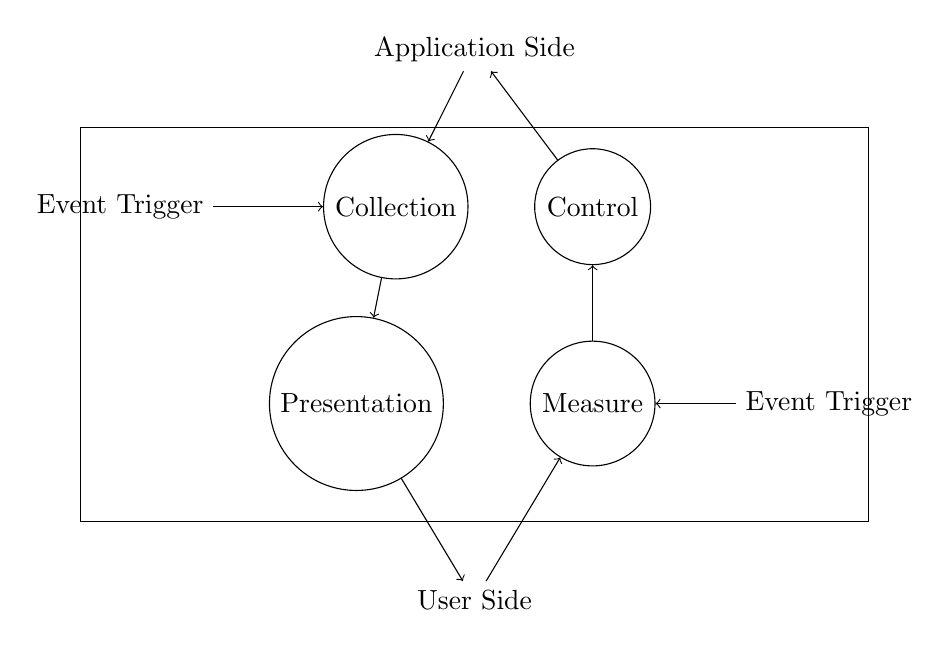
\begin{tikzpicture}
		
		\node[rec,minimum width = 10cm,minimum height = 5cm,xshift = 0.5cm]() {};
		\node[circ,xshift=-0.5cm,yshift = 1.5cm](Collection) {Collection};
		\node[circ,xshift=-1cm,yshift=-1cm](Presentation) {Presentation};
		\node[circ,xshift=2cm,yshift=-1cm](Measure) {Measure};
		\node[circ,xshift=2cm,yshift=1.5cm](Control) {Control};
		\node[yshift=3.5cm,xshift=0.5cm](Application) {Application Side};
		\node[yshift=-3.5cm,xshift=0.5cm](User) {User Side};\pause
		
		\draw[->] (User) -- (Measure); \pause
		\node[xshift=5cm,yshift=-1cm](TriggerUser) {Event Trigger};
		\draw[->] (TriggerUser) -- (Measure);\pause
		\draw[->] (Measure) -- (Control); \pause
		\draw[->] (Control) -- (Application);\pause
		
		\draw[->] (Application) -- (Collection);\pause
		\node[xshift=-4cm,yshift=1.5cm](TriggerApp) {Event Trigger};
		\draw[->] (TriggerApp) -- (Collection);\pause
		\draw[->] (Collection) -- (Presentation);\pause
		
		\draw[->] (Presentation) -- (User);
				
		\end{tikzpicture}
	\end{figure}
	
\end{frame}

\section{How it works?}
\begin{frame}{How it works?}
	Figure 3 goes here. with a pager. that animates the process of communication of interactors
\end{frame}

\section{Formal Definition of an Interactor}
\begin{frame}{Formal Definition of an Interactor}
	An block goes here. With title and description with defintion.Would need mathematical latex to notate the definitions.
\end{frame}


\end{document}
